\section{Experimental Results}
The following section describes the experimental results for direct and trained quantization of All-CNNs on three datasets.

\subsection{Experimental Setup}
For experimental evaluation, we apply the proposed methods on All-Convolutional Networks for the Datasets CIFAR-10 \cite{Krizhevsky2009}, CIFAR-100 and SVHN \cite{netzer2011reading}. We use All-Convolution Network model All-CNN-C from \cite{Springenberg2015} for evaluation. The CNN Architecture summed up in table \ref{tab:allconv} consists of nine convolution layers and a global average pooling layer. Due to the similar filter-width and height the number of weights in the convolution layers mainly depends on the filter-depths. The number of operations also depends on the layer-output dimensions. However, it needs to be 
noted that the proposed technique is neither architecture nor dataset bound. 

\begin{table}[ht!]
  \caption{All-CNN-C Architecture and the number of weights and MAC-operations for one forward computation with batch-size one.}
  \label{tab:allconv}
  \begin{tabular}{c|c|c|c}
    \toprule
    	\textbf{Layer (WxH) }& \textbf{Output Dim. (WxHxD) }& \textbf{\#Weights} & \textbf{\#MACs} \\
    \midrule
    	Input &  32x32x3 & - & - \\
    	Conv. 3x3 &  32x32x96 & 2K & 2.3M \\
    	Conv. 3x3 &  32x32x96 & 83K & 74.6M\\
    	Conv. 3x3 &  32x32x96 & 83K & 74.6M\\
    	Pooling 2x2 &  16x16x96 & - & -\\
    	Conv. 3x3 &  16x16x192 & 165K & 32.5M\\
    	Conv. 3x3 &  16x16x192 & 332K & 65M\\
    	Conv. 3x3 &  16x16x192 & 332K & 65M\\
    	Pooling 2x2 &  8x8x192 & - & -\\
    	Conv. 3x3 &  8x8x192 & 332K & 11.9M\\
    	Conv. 1x1 &  8x8x192 & 37K & 2.4M\\
    	Conv. 1x1 &  8x8x10 & 2K & 0.1M\\
    	Pooling 8x8 &  10 & - & -\\
            \midrule
    	\textbf{Total}&  - & \textbf{1386K} & \textbf{329.7M} \\
  \bottomrule
\end{tabular}
\end{table}

For the three datasets, we use the predefined training and test sets. For the floating point baselines we trained the CNN for 350 epochs with initial \highlight{learning rate $10^{-3}$} multiplied by a fixed multiplier after epochs 200 and 300. To avoid over-fitting, we use dropout with dropout rate 0.5 after layers. In contrast to the original All-CNN paper \cite{Springenberg2015}, the models are not regularized by weight decay to avoid interfering with the studied regularization methods. In terms of data augmentation we only apply horizontal flipping and random shifting by a maximum of 3 pixels. 

\subsection{Performance Analysis}
We evaluate the performance of the proposed method comparing the test accuracy of the original network with the resulting accuracies after direct and trained quantization. For the tables \ref{tab:res_CIFAR10}, \ref{tab:res_CIFAR100} and \ref{tab:res_SVHN}, we make use of the abbreviations in table \ref{tab:metrics}.
We aim to achieve high compression rates in terms of weight memory while maintaining high test accuracy. \highlight{In addition to bit-width reduction we also consider the resulting sparsity as an important factor for possible further compression.} Assuming skipping of multiplications with 0 weights, sparsity also reduces the amount of required MAC-operations for forward computation.\footnote{The number of skipped MACs due to a pruned weight depends on the layer-input dimensions. Therefore sparsity in weights is unequal to sparsity in MACs.} \highlight{For all experiments except the two marked, bit-width for activations is 32-bit Fixed Point}.
%\caj{Why is the sparsity of weights different from the sparsity of MACs in the tables?}
%\cmw{This derives from the reuse of weights and the input dimensions. Say in layer 1 a weight is 0, it accounts for 32x32 multiplications, while a weight in layer 5 for 16x16 multiplications.}
%\todo[inline]{
%comparison to other methods (improvement)}
%\todo[inline]{Results like in IMAGE shown implementing the SQNR and then Retraining (necessity of the approach)
%\newline comparison to other methods (improvement)
%\newline Relationship Accuracy, Loss during retraining
%\newline influence of the lambda parameter
%\newline influence of learning rate
%}




\subsubsection{CIFAR-100}


CIFAR-100 is an image classification dataset consisting of a training set of 50000 and a test set of 10000 32$\times$32 color images representing 100 different categories such as airplanes, automobiles, birds, cats, deers,dogs, frogs, horses, ships and trucks \cite{Krizhevsky2009}. The training batches contain exactly 5000 images from each class. Table \ref{tab:res_CIFAR10} shows the resulting accuracies after fine-tuning with 200 epochs of WQR with $\lambda_2 = epoch\times 10$. In addition $\lambda_1$ is set to 100 starting at epoch 150. This setup is not optimal for all configurations, as in some cases training with only QR would be sufficient, but it allows using the same parameterization for each iteration increasing comparability. Compared to a full implementation (32-bit), the proposed layer-wise quantization (DFP-lw) saves $\sim$4-8$\times$ in terms of weight memory and has an accuracy loss by $\sim$0.1-4.5\%. Compared to the reduced equal bit-width quantization, the proposed layer-wise quantization has higher sparsity and smaller weight memory. 

\begin{table*}[ht!]
\caption{Results in comparison to floating point baseline of All-CNN for CIFAR-100 (CR=Compression ratio)}
%  \caj{Is the activation bit-width 8bit for all experiments? If yes, we should write this; if not, we should explain what the activation bit-width is in those cases. Anyway, the footnote is the wrong place to explain this. }
%  \cmw{Added explanation in first paragraph section 4.2}
  \label{tab:res_CIFAR100}
  \begin{tabular}{cc|ccc|cc|ccc}
\toprule
    	$b_n$&Type&$W_{mem}$\lbrack$Bit$\rbrack$$&CR& Sparsity$\lbrack\%\rbrack$ & non-0 MACs & MAC Sparsity$\lbrack\%\rbrack$ & $acc_{tr}\lbrack\%\rbrack$ & $acc_{init}\lbrack\%\rbrack$ & $acc_{M_q}\lbrack\%\rbrack$\\
\hline
 		32 bit & float & 44344K & 1 &  0 & 329.7M & 0 & 83.24 & 63.03 &  \textbf{63.03} \\
\hline
 		8 bit & DFP-eq & 11086K & 4 & 5.8 & 304.8M & 7.6 &83.5&62.43&\textbf{62.99} \\
 		7 bit & DFP-eq & 9700K & 4.6 & 11.5 & 280.3M & 15 &82.65&61.86&\textbf{62.38}\\
 		6 bit & DFP-eq & 8314K & 5.3 & 21.9 & 234.1M & 29 & 81.02&58&\textbf{61.19}\\
 		5 bit & DFP-eq & 6928K & 6.4 & 38.9 & 161M & 51.2 & 76.99&43.72&\textbf{59.54}\\
\hline
       	$\lbrack$9	9	9	9	6	5	7	9	9$\rbrack$ & DFP-lw & 9485K & 4.7 & 14.6 & 289.5M & 12.2 &83.44&62.90&\textbf{62.93}\\
       	$\lbrack$9	9	9	9	5	5	5	9	9$\rbrack$ & DFP-lw & 8490K & 5.2 & 23.2 & 279.2M & 15.3 &82.45&62.45&\textbf{62.64}\\
       	$\lbrack$9	9	9	5	4	4	5	9	9$\rbrack$ & DFP-lw & 7163K & 6.2 & 36.4 & 243.4M & 26.2 &80.76&61.70&\textbf{62.29}\\ 	
        $\lbrack$9	6	5	5	3	3	4	7	9$\rbrack$ & DFP-lw & 5513K & 8.0 & 60.4 & 133.6M & 59.5 &73.76&55.69&\textbf{58.58}\\
\hline
 		4 bit & Po2-eq & 5543K & 8 & 18.3 & 255.2M & 22.6 & 79.47 & 51.27 & \textbf{60.94}\\
\hline
\end{tabular}
\end{table*}

\begin{table*}[ht!]
  \caption{Results in comparison to floating point baseline of All-CNN for CIFAR-10}
  \label{tab:res_CIFAR10}
  \begin{tabular}{cc|ccc|cc|ccc}
\hline
    	$b_n$&Type&$W_{mem}\lbrack$Bit$\rbrack$&CR& Sparsity$\lbrack\%\rbrack$ & non-0 MACs & MAC Sparsity$\lbrack\%\rbrack$ & $acc_{tr}\lbrack\%\rbrack$ & $acc_{init}\lbrack\%\rbrack$ & $acc_{M_q}\lbrack\%\rbrack$\\
\hline
 		32 bit & float & 43791K & 1 & 0 & 329.7M & 0 & 96.69 &  90.83 &  \textbf{90.83} \\
\hline
 %		all 5 bit & DFP & 6842K & 6.4 & 27.4 & 185.9M & 43.4 & 95.82 & 87.13 & \textbf{89.92}\\
  		8 bit & DFP-eq\footnotemark & 10947K & 4 & 4.2 & 303.5M & 7.6 & 96.64 & 90.65 & \textbf{90.85}\\
 		4 bit & DFP-eq & 5474K & 8 & 42.3 & 140.7M & 57.2 & 94.4 & 44.47 & \textbf{88.63}\\
\hline
              	$\lbrack$8 8 8 5 4 4 3 8 8$\rbrack$ & DFP-lw$^4$ &5929K& 7.38& 36.8 & 243M & 26 & 96.49 & 90.14 &\textbf{90.81}\\
              	$\lbrack$7 7 7 4 4 3 3 7 7$\rbrack$ & DFP-lw &5432K& 8.1&46.1&203.9M&37.9&96.01&90.07&\textbf{90.32}\\
 %		$\lbrack$6 6 4 4 3 3 3 5 6$\rbrack$ & DFP &4690K& 9.3&57.2&126.6M&61.4&95.16&87.79&\textbf{89.53}\\

 %		5 bit & Po2 & 6842KBit  & 6.4 & 0 & 327.8M & 0.01&96.22&90.45&75.56&\textbf{90.21}\\
 \hline
 		4 bit & Po2-eq & 5474K & 8 & 13.2 & 255.9M &  22.1 &96.13&76.73&\textbf{90.18}\\
 %		all 5 bit & DFP & 6842K & 6.4 & 27.4 & 185.9M & 43.4 & 95.82 & 87.13 & \textbf{89.92}\\
\hline
\end{tabular}
\end{table*}

\begin{table*}[ht!]
  \caption{Results in comparison to floating point baseline of All-CNN for SVHN}
  \label{tab:res_SVHN}
  \begin{tabular}{cc|ccc|cc|ccc}
\hline
    	$b_n$&Type&$W_{mem}\lbrack$Bit$\rbrack$&CR& Sparsity$\lbrack\%\rbrack$ & non-0 MACs & MAC Sparsity$\lbrack\%\rbrack$ & $acc_{tr}\lbrack\%\rbrack$ & $acc_{init}\lbrack\%\rbrack$ & $acc_{M_q}\lbrack\%\rbrack$\\
\hline
 		32 bit & float & 43791K & 1 & 0 & 329.7M & 0 & 97.70 & 95.84 & \textbf{95.84} \\
\hline
% 		all 5 bit & DFP & 6842K & 6.4 & 27.4 & 185.9M & 43.4 & 95.82 & 87.13 & \textbf{89.92}\\
 		4 bit & DFP-eq & 5474K & 8 & 43.5 & 166.8M & 49.2 & 96.27 & 86.17 & \textbf{95.37}\\
\hline
  %     	$\lbrack$7 7 6 4 3 3 4 7 6$\rbrack$ & DFP-lw &5347K& 8.2&54.1&190.9M&41.8&96.69&95.57&\textbf{95.89}\\
 		$\lbrack$6 4 4 3 3 3 4 5 6$\rbrack$ & DFP-lw &4690K& 9.3&62.7&126.6M&63.2&96.43&95.03&\textbf{95.89}\\
         $\lbrack$5 4 4 3 3 3 3 3 3$\rbrack$ & DFP-lw &4276K& 10.23&70.5&116.7M&64.4&95.52&89.86&\textbf{95.36}\\
\hline
 %		5 bit & Po2 & 6842KBit  & 6.4 & 0 & 327.8M & 0.01&96.22&90.45&75.56&\textbf{90.21}\\
 		4 bit & Po2-eq & 5474K & 8 & 17.0 & 272.8M & 16.9  &97.02&91.93&\textbf{96.02}\\
\hline
\end{tabular}
\end{table*}



In addition, figure \ref{fig:lw_100} depicts the results of trained quantization in comparison to direct quantization. We can see that retraining with QR and WQR in all cases increases classification accuracy in comparison to direct quantization.

\begin{figure}[ht!]
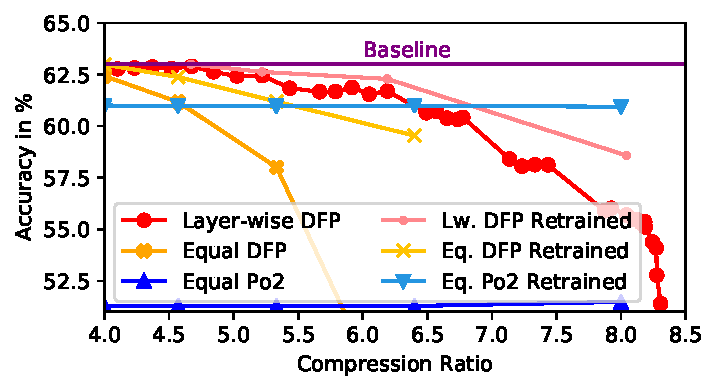
\includegraphics[width=\columnwidth]{img/res100.pdf}
\caption{Results for direct and trained DFP and Po2 quantization with equal bit-widths on ALL-CNN for CIFAR-100. For DFP also Layer-wise Precision Scaling with direct and trained quantization is illustrated.}\label{fig:lw_100}
\end{figure}
Comparing equal bit-width quantization with Layer-wise Precision Scaling for DFP datatype, we can see that for similar compression ratios, equal bit-width (DFP-eq) never reaches the accuracy of Layer-wise Precision Scaling (DFP-lw), even when retraining with WQR/QR is applied. For Po2 quantization we found equal 4 bit quantization (Po2-eq) the most effective method as higher bit-widths did not increase accuracy and Layer-wise Precision Scaling for lower than 4 bit leads to drastic accuracy drop.


\subsubsection{CIFAR-10}
CIFAR-10 is a benchmark image classification dataset equal to CIFAR-100 in terms of image and dataset sizes, which instead of 100 classes divides the images into 10 classes. We use the same training method as for CIFAR-100. The results for trained quantization of All-CNN for CIFAR-10 are shown in table \ref{tab:res_CIFAR10}. To allow comparing to other works for the two marked configurations, we also quantized the activations to 8-bit DFP. In contrast to ALL-CNN for CIFAR-100, for this dataset higher compression rates can be achieved. For Compression Ratio $\sim 8$, DFP with Layer-wise Precision Scaling (DFP-lw) gives lowest accuracy degradation of $0.51$ percentage points. For equal bit-with quantization Po2 outperforms DFP by $1.55$ percentage points. For Compression Ratio $7.38$ classification accuracy of DFP with Layer-wise Precision Scaling is only $0.01$ percentage points below the floating point baseline.

\begin{figure}[ht!]
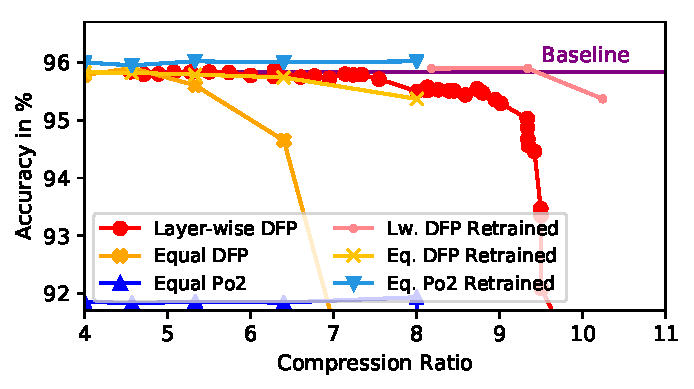
\includegraphics[width=\columnwidth]{img/ressvhn.pdf}
\caption{Results for direct and trained DFP and Po2 quantization with equal bit-widths on ALL-CNN for SVHN. For DFP also Layer-wise Precision Scaling with direct and trained quantization is illustrated.}\label{fig:lw_svhn}
\end{figure}
\subsubsection{SVHN}
The SVHN image classification dataset consists of 694K 32$\times$32 color images for training and 26K images for testing. The images represent digits form 0 to 9.
Similarly to CIFAR-100 and CIFAR-10 we perform Layer-wise Precision Scaling and retraining with WQR and QR for model compression. The results are shown in table \ref{tab:res_SVHN} and figure \ref{fig:lw_svhn}. For the SVHN dataset at Compression Ratio $\sim 8$, Po2 quantization and DFP with Layer-wise Precision Scaling both outperform the original baseline model.

\vspace{1ex}
Comparing the results for the datasets CIFAR-100, CIFAR-10 and SVHN, we can conclude that the attainable Compression Ratio for lossless trained quantization with QR/WQR not only depends on the selected datatype and bit-widths, but also on the selected datasets. 
\highlight{While for CIFAR-10 and SVHN, lossless trained quantization achieves Compression Ratio 8.0 and 9.4 respectively, for CIFAR-100 the maximum Compression Ratio is 4.7 for lossless compression. 
In the case of CIFAR-100 further increasing Compression Ratio up to 8.0 reduces accuracy by 2.09 percentage points. In contrast to this trade-off, stronger compression for CIFAR-10 and SVHN immediately leads to drastic accuracy reduction.
We suspect that this difference can be explained by the relation between complexity of the dataset and the selected network architecture. To better understand this relation, in future work the techniques have to be applied for further datasets and network topologies.}

%\highlight{When applying the trained quantization with QR/WQR on the selected network for CIFAR-100, lossless compression for compression rates up to 4.7 is possible. Further increasing the compression rate to 8.0, leads to a reduction in accuracy of 2.09 percentage points.
%For the datasets CIFAR-10 and SVHN on the other hand, lossless compression is still possible for high Compression Rates (8.0 and 9.4 respectively). We can conclude that the attainable Compression Ratio for lossless trained quantization with QR/WQR not only depends on the selected datatype and bit-widths, but also on the selected datasets. 
%While for SVHN and CIFAR-10 the Compression Rates can be used in all cases,
%In addition to that, for CIFAR-100 the trade-off between Compression Rate and accuracy allows the adaptation of bit-widths and datatypes to the requirements of the application.}

While with DFP lossless compression can always be achieved, Po2 quantization can sometimes lead to slight performance degradation. Layer-wise Precision Scaling turns out to be more effective for DFP than for Po2. \highlight{Po2 quantization still reaches maximum accuracy at uniform 4 bit bit-width while achieving higher accuracy than uniform 4 bit and even 5 bit DFP quantization.}

\footnotetext{8-bit DFP for activations}
\section{Comparison with Related Work}
The proposed method of Weighted Quantization-Regularization presents a novel technique for trained quantization of DNNs. However in some works performing weight-binarization similar regularization methods are used to achieve weights with values `$+$1' or `$-$1' \cite{Tang2017}. Today trained quantization is mostly performed by stochastic rounding during training \cite{Courbariaux2014, Courbariaux2015, Gysel2016, Gupta2015a}. Gupta et al. \cite{Gupta2015a} apply stochastic training for CIFAR-10 dataset to achieve Fixed Point quantization to 16-bit and 12-bit. Their accuracy is reduced by 0.8 and 4.2 percentage points respectively compared to the floating point baseline. In comparison to that with our method we reach 8-bit DFP quantization without any performance drop.

Courbariaux et al. \cite{Courbariaux2014} perform quantization based on stochastic round for 10bit Dynamic Fixed Point weights and activations. \highlight{Their accuracy drops in comparison to the baseline networks 3.14 percentage points for CIFAR-10 and 2.58 percentage points for SVHN since in contrast to us, they also perform weight-update with 12-bit DFP which decreases comparability. For our CIFAR-10 and SVHN network we experimentally also applied 8-bit DFP for weights and activations, and found that accuracy even increased after QR/WQR retraining.} Gysel et al. \cite{Gysel2016} use their CAFFE-based tool Ristretto for Layer-wise Precision Scaling and fine-tuning with stochastic rounding. On CIFAR-10 their accuracy lies 0.3\% below the floating point baseline accuracy, when quantizing not only weights but also activations to 8 bit DFP. By applying Layer-wise Precision Scaling we are able to increase compression ratio from $4$ to $7.38$ and after QR/WQR-retraining achieve equal to baseline accuracy while inducing higher sparsity due to the stronger compression.
Other than fine-tuning with stochastic rounding, Zhou et al. \cite{Zhou2017a} presented an incremental retraining method to perform Power-of-two weight quantization. They achieve lossless 5-bit/4-bit quantization for several DNNs for the ImageNet dataset. Even for lower bit-rates incremental quantization achieves state-of-the-art results. Even though this method seems highly promising, in contrast to our work, it is only verified to work for power-of-two quantization.
%Deep Compression achieves high compression rate on AlexNet and VGG but the high compression rate is mainly based on pruning and encoding of the fully connected layer at the end of the network for Convolutional layers they use 8 bit but not fixed quantization scheme but clustering for weight sharing

%SQNR presents a predictive method for equidistant quantization but does only take the network archtitecture and not the actual data, Adaptive Method sadly no means to compare but don't apply retraining


\section{Conclusion}
% {\color{blue}
% Main points:

% \begin{itemize}
% \item DFP is preferable to Po2, because
% \begin{itemize}
% \item it is as good as or better than Po2 most of the time;
% \item it can reach floating point accuracy when increasing the bitwidth;
% \item it does not require retraining (retraining improves the accuracy but for Po2 it is necessary;
% \end{itemize}
% \item In a few, special cases with low bit-width Po2 is slightly better than DFP;
% \begin{itemize}
% \item it can be better for hardware, since Po2 means only shifting instead of multiplying
% \end{itemize}
% \item WQR/QR allows fine-tuning for weights to any quantization scheme (data-type) increasing accuracy in comparison to "direct quantization"  (quantization) without retraining. 
% \item WQR/QR also works for non-uniform bit-widths (Layer-wise Precision Scaled) and in combination we achieve high compression ratio and high accuracy (WQR/QR)
% \item For ALL-CNN for CIFAR-10
% for example reaches lossless compression up to compression ratio 7.34 with DFP and Layer-Wise Precision Scaling.
% \item Compared to the 32bit floating point baseline in the All-CNN network DFP with WQR and DFP we see a weigh memory compaction of 8.0-8.2x and a MAC sparsity of 37.9-59.5\% in the benchmark tasks. For these cases with maximal compaction we observe between 0.51-4.45 percentage points reduction of classification accuracy and in one case (SVHN) even an accuracy increase of 0.05 percentage points. 
% \item WQR is not a stand-alone tool but can be combined with other techniques and is complementary to those.
% \item It has some limitations when applied to very low bit-widths (hence combination with stochastic rounding method would be future work)
% \end{itemize}}

We propose Quantization-Regularization (QR) and Weighted QR (WQR) as techniques for improving accuracy after bit-width reductions inflicted by a quantization scheme. WQR/QR allow fine-tuning for weights in any quantization scheme and also works for non-uniform bit-widths (Layer-wise Precision Scaling). For ALL-CNN with the CIFAR-10 benchmark WQR reaches lossless compression up to a ratio of 7.38x with DFP and Layer-wise Precision Scaling.
Compared to the 32bit floating point baseline in the All-CNN network, WQR with DFP obtains a weight memory compaction of 8.0$\times$-10.23$\times$ and a MAC sparsity of 37.9\%-64.4\% in the benchmark tasks. For these cases with maximal compaction we observe between 0.48-4.45 percentage points reduction of classification accuracy. A high MAC sparsity benefits HW implementations because it potentially reduces the number of multiply-accumulate operations.

Note, that WQR/QR is not a stand-alone tool, but can be combined with other techniques and is typically complementary to those.
We have observed, that it has some limitations when applied to very low bit-widths; hence, its combination with stochastic rounding methods is considered as future work.

Furthermore, we have studied two quantization schemes, Dynamic Fixed Point (DFP) and Power-of-two (Po2), and we find that DFP is usually preferable to Po2 because it is as good as or better than Po2 in most cases, it can reach floating point accuracy when increasing bit-width, and it does not necessarily require retraining (retraining improves accuracy but for Po2 it is absolutely necessary). However, in a few special cases with low bit-width Po2 is slightly better and it might be preferred for HW implementations because it requires only shift operations instead of multiplications. Thus, when an optimized HW implementation is developed, Po2 could be considered as a useful option.

%We have presented Weighted Quantization-Regularization, a method for trained quantization of Deep Neural Networks and evaluated the properties of Power-of-two and Dynamic Fixed Point quantization with uniform bit-widths and Layer-wise Precision Scaling. % and compared their behavior when applying Layer-wise Precision Scaling and fine-tuning with Weighted Quantization-Regularization.


%The two presented datatypes not only reduce weight memory but are also hardware-friendly weight representations which can help increase computational efficiency. For Dynamic Fixed Point quantization, Layer-wise Precision Scaling in combination with Weighted Quantization-Regularization is an effective method to compress weight memory up to a factor of 10 in All Convolutional Networks. When applying equal bit-width quantization for Power-of-two or Dynamic Fixed Point datatype, retraining with Weighted Quantization-Regularization is an effective method to minimize accuracy degradation. While with the Dynamic Fixed Point datatype the resulting accuracy can be improved up to the original baseline accuracy by increasing the bit-width, Power-of-two quantization already reaches best accuracy for a bit-width of 4. Finally we don't see Weighted Quantization-Regularization as a standalone quantization technique, but we are positive that it could boost the performance of current state-of-the-art methods when applied as regularizer.



%Results exist for \cite{Shin2017}
